\section*{Aufgabe 3: }
Die Partitionierung des Raumes kann auch durch ein Prisma mit einem gleichschenkligen Dreieck als Grundfläche geschehen. Dann kann die Aufteilung des Raumes von dem Prisma stattfinden, indem die Höhe und Grundseite des Dreiecks halbiert werden und das daraus resultierende Prisma wie in der folgenden Abbildung viermal positioniert wird.
\begin{figure}[H]
  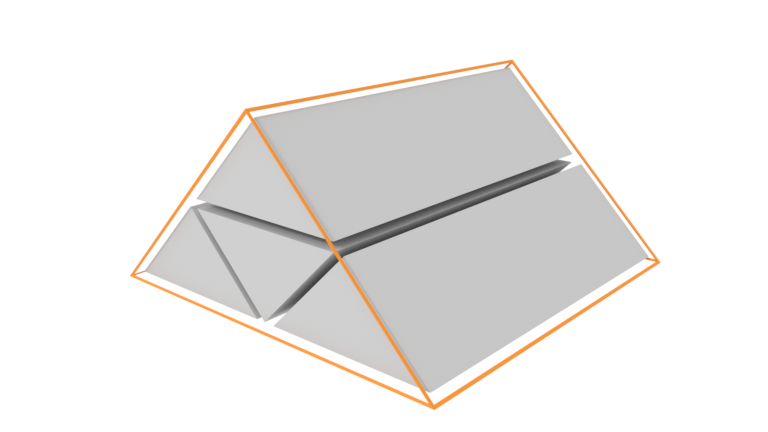
\includegraphics[width=0.7\textwidth]{prism}
\end{figure}